\chapter{Tools and Frameworks}
\label{chap:tools}

This chapter describes how the components introduced in Chapter~2 are assembled into a single pipeline: COLMAP-based preprocessing, Nerfstudio training with Splatfacto, optional Hub-hosted depth and segmentation models (Section~\ref{sec:huggingface}), and lightweight geometry utilities. Chapter~\ref{chap:methodology} documents the method-specific extensions applied on top of this stack.

\section{Data preparation}
\label{sec:data_preparation}

The SfM stages were outlined in Chapter~2; here the focus is on the Nerfstudio wrapper around COLMAP. Preprocessing starts with \texttt{ns-process-data images} (or \texttt{video}), implemented by \texttt{Colmap\-Converter\-To\-Nerfstudio\-Dataset} and \texttt{run\_colmap} under \filepath{nerfstudio/process\_data/}. The helper invokes the external \texttt{colmap} binary in sequence: SIFT \texttt{feature\_extractor} (default camera model \texttt{perspective}), a matcher (\texttt{vocab\_tree}, \texttt{exhaustive}, or \texttt{sequential} for ordered video), incremental \texttt{mapper}, and optionally \texttt{bundle\_adjuster} for intrinsic refinement. The resulting folder contains \filepath{colmap/sparse/} (with COLMAP-native \filepath{points3D.bin} or \filepath{points3D.txt}), a converted \filepath{sparse\_pc.ply} used to seed Gaussian means, and \filepath{transforms.json}.

The manifest stores global intrinsics (\texttt{fl\_x}, \texttt{fl\_y}, \texttt{cx}, \texttt{cy}, distortion coefficients, image dimensions). Each frame entry lists a \texttt{file\_path} and a $4\times4$ camera pose stored as \texttt{transform\_matrix}. Dataparsers convert these fields into batched \texttt{Cameras} tensors. Existing COLMAP reconstructions can be ingested without re-running SfM; packaged benchmark scenes are available via \texttt{ns-download-data}.

\section{Nerfstudio and Splatfacto}
\label{sec:splatfacto_gsplat}

Nerfstudio \cite{tancik2023nerfstudio} organizes experiments behind typed \code{@dataclass} configs, swappable \code{DataParser}/\code{DataManager}/\code{Model} components, and a \code{Pipeline} that forwards \code{get\_train\_loss\_dict} to a shared trainer. User commands (\code{ns-process-data}, \code{ns-train}, \code{ns-export}, \code{ns-viewer}, among others) are registered as console scripts in \code{pyproject.toml}.\footnote{\url{https://docs.nerf.studio/}}

\begin{figure}[H]
    \centering
    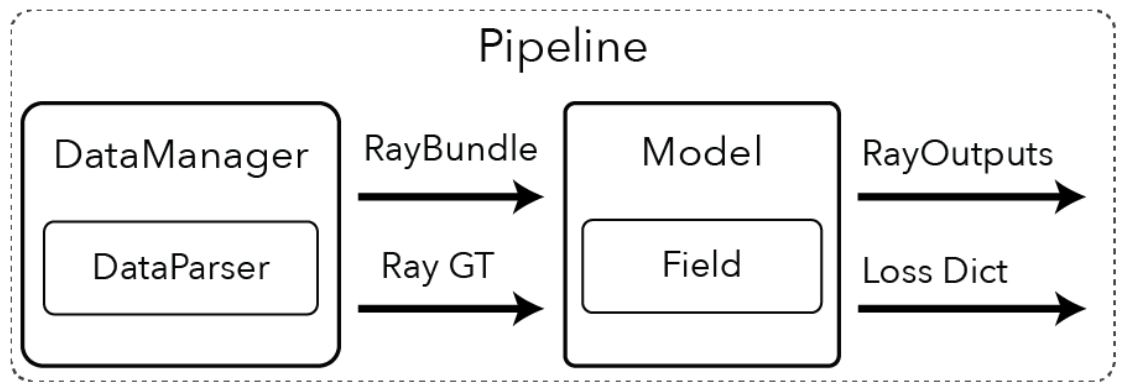
\includegraphics[width=0.85\textwidth]{images/nergstudio.png}
    \caption[Nerfstudio training pipeline]{Nerfstudio training flow: a \code{DataParser} loads disk data, a \code{DataManager} batches viewpoints, and a \code{Model} returns losses. Splatfacto swaps ray bundles for full-frame \code{Cameras} and replaces the MLP \code{Field} with explicit Gaussian parameters.}
    \label{fig:nerfstudio_pipeline}
\end{figure}

The method used throughout this thesis is \textbf{Splatfacto}, the 3D Gaussian Splatting implementation in Nerfstudio \cite{kerbl2023gaussian}. Scene geometry is stored as explicit per-Gaussian tensors (means, covariances, spherical-harmonic colors, opacities) inside \code{SplatfactoModel}; rendering and optimization use \code{FullImageDataManager}, which supplies undistorted full-frame RGB at each step. Differentiable rasterization is delegated to \code{gsplat}, whose CUDA kernels are JIT-compiled on first execution atop PyTorch.

Gaussian means are initialized from the sparse point cloud (\filepath{sparse\_pc.ply}, derived from COLMAP triangulation) when \filepath{transforms.json} is present. Trained checkpoints can be inspected in the Nerfstudio web viewer or exported to \textbf{SuperSplat} \cite{supersplat2024} for interactive inspection of Gaussian centers, ellipsoid geometry, and splat rendering (\url{https://superspl.at/}).

\section{Pretrained models (Hugging Face Hub)}
\label{sec:huggingface}

By default, the pretrained models invoked in this thesis are not vendored as local checkpoints inside the repository. Instead, weights and configuration files are resolved at runtime through the \textbf{Hugging Face Hub}\footnote{\url{https://huggingface.co}}. Each model is identified by a repository id and loaded with \texttt{from\_pretrained(...)}, which downloads or reuses a cached snapshot on first use. Examples include \codeid{depth-anything/da3metric-large} and \codeid{IDEA-Research/grounding-dino-base}.

\subsection{Depth Anything 3 (metric depth)}
Monocular metric depth for supervision and visualization is provided by \texttt{Depth\-Anything3} via \texttt{from\_pretrained} in \filepath{nerfstudio/models/da3\_depth.py}. The default checkpoint is \textbf{DA3METRIC-LARGE} (\codeid{depth-anything/da3metric-large}). During preprocessing (\texttt{ns-process-data} with DA3 depth export) or inside Splatfacto when \texttt{loss=depth}, the wrapper passes each RGB frame and the COLMAP focal length in pixels to obtain a dense depth map in meters.

\subsection{Grounding DINO and SAM~2 (segmentation)}
Object-centric masks rely on two additional Hub-hosted models, implemented in \filepath{nerfstudio/models/sam2\_semantics.py}:
\begin{itemize}
    \item \textbf{Grounding DINO} is loaded via \texttt{transformers} (\texttt{Auto\-Processor} and \texttt{Auto\-Model\-For\-Zero\-Shot\-Object\-Detection.from\_pretrained}), using \codeid{IDEA-Research/grounding-dino-base} by default unless overridden in the Splatfacto config.
    \item \textbf{SAM~2} is loaded through \texttt{SAM2\-Image\-Predictor.from\_pretrained} with a configurable Hub id (for example \codeid{facebook/sam2-hiera-large}), then prompted with boxes from Grounding DINO to obtain per-view binary masks.
\end{itemize}
The same Hub id pins weights across machines; Nerfstudio handles orchestration and loss integration only.

\section{Auxiliary tools}

In this thesis, Open3D \cite{zhou2018open3d} is used to export and inspect the learned B\'ezier surfaces. At the end of training (\texttt{export\_bezier\_meshes}), each patch is sampled on a uniform $(u,v)$ grid; the resulting 3D points are the mesh vertices, and a regular grid triangulation yields triangle faces. Open3D assembles this as a \texttt{TriangleMesh} and writes PLY files (outer, inner, and shell variants when applicable), which can then be opened in any 3D viewer for qualitative inspection. Nerfstudio also uses Open3D elsewhere (e.g.\ loading \filepath{sparse\_pc.ply} for Gaussian initialization), but that path is unrelated to the B\'ezier surface exports described here.

